% bei Standalone in documentclass noch:
% \RequirePackage{luatex85}

\documentclass[captions=tableheading, titlepage= firstiscover, parskip = half , bibliography=totoc]{scrartcl}
%paper = a5 für andere optinen
% titlepage= firstiscover
% bibliography=totoc für bibdateien
% parskip=half  Veränderung um Absätze zu verbessern

\usepackage{scrhack} % nach \documentclass
\usepackage[aux]{rerunfilecheck}
\usepackage{polyglossia}
\usepackage[style=numeric, backend=biber]{biblatex} % mit [style = alphabetic oder numeric] nach polyglossia
\addbibresource{lit.bib}
\setmainlanguage{german}

\usepackage[autostyle]{csquotes}
\usepackage{amsmath} % unverzichtbare Mathe-Befehle
\usepackage{amssymb} % viele Mathe-Symbole
\usepackage{mathtools} % Erweiterungen für amsmath
\usepackage{fontspec} % nach amssymb
% muss ins document: \usefonttheme{professionalfonts} % für Beamer Präsentationen
\usepackage{longtable}

\usepackage[
math-style=ISO,    % \
bold-style=ISO,    % |
sans-style=italic, % | ISO-Standard folgen
nabla=upright,     % |
partial=upright,   % /
]{unicode-math} % "Does exactly what it says on the tin."
\setmathfont{Latin Modern Math}
% \setmathfont{Tex Gyre Pagella Math} % alternativ

\usepackage[
% die folgenden 3 nur einschalten bei documenten
locale=DE,
separate-uncertainty=true, % Immer Fehler mit ±
per-mode=symbol-or-fraction, % m/s im Text, sonst \frac
]{siunitx}

% alternativ:
% per-mode=reciprocal, % m s^{-1}
% output-decimal-marker=., % . statt , für Dezimalzahlen

\usepackage[
version=4,
math-greek=default,
text-greek=default,
]{mhchem}

\usepackage[section, below]{placeins}
\usepackage{caption} % Captions schöner machen
\usepackage{graphicx}
\usepackage{grffile}
\usepackage{subcaption}

% \usepackage{showframe} Wenn man die Ramen sehen will

\usepackage{float}
\floatplacement{figure}{htbp}
\floatplacement{table}{htbp}

\usepackage{mhchem} %chemische Symbole Beispiel: \ce{^{227}_{90}Th+}


\usepackage{booktabs}

 \usepackage{microtype}
 \usepackage{xfrac}

 \usepackage{expl3}
 \usepackage{xparse}

 % \ExplSyntaxOn
 % \NewDocumentComman \I {}  %Befehl\I definieren, keine Argumente
 % {
 %    \symup{i}              %Ergebnis von \I
 % }
 % \ExplSyntaxOff

 \usepackage{pdflscape}
 \usepackage{mleftright}

 % Mit dem mathtools-Befehl \DeclarePairedDelimiter können Befehle erzeugen werden,
 % die Symbole um Ausdrücke setzen.
 % \DeclarePairedDelimiter{\abs}{\lvert}{\rvert}
 % \DeclarePairedDelimiter{\norm}{\lVert}{\rVert}
 % in Mathe:
 %\abs{x} \abs*{\frac{1}{x}}
 %\norm{\symbf{y}}

 % Für Physik IV und Quantenmechanik
 \DeclarePairedDelimiter{\bra}{\langle}{\rvert}
 \DeclarePairedDelimiter{\ket}{\lvert}{\rangle}
 % <name> <#arguments> <left> <right> <body>
 \DeclarePairedDelimiterX{\braket}[2]{\langle}{\rangle}{
 #1 \delimsize| #2
 }

\setlength{\delimitershortfall}{-1sp}

 \usepackage{tikz}
 \usepackage{tikz-feynman}

 \usepackage{csvsimple}
 % Tabellen mit \csvautobooktabular{"file"}
 % muss in table umgebung gesetzt werden


% \multicolumn{#Spalten}{Ausrichtung}{Inhalt}

\usepackage{hyperref}
\usepackage{bookmark}
\usepackage[shortcuts]{extdash} %nach hyperref, bookmark

\newcommand{\ua}[1]{_\symup{#1}}
\newcommand{\su}[1]{\symup{#1}}


\begin{document}

\section{Auswertung}

Im Folgendem werden die Messergebnisse ausgewertet und auf geeignete Weise
visualisiert.
Die verwendete Schaltung hatte die folgenden Daten.

\begin{align*}
  L &= \SI{3,53\pm 0,03}{\milli\henry} \\
  C &= \SI{5,015\pm 0,015}{\nano\farad} \\
  R_1 &= \SI{30,3\pm 0,1}{\ohm} \\
  R_2 &= \SI{271,6\pm 0,3}{\ohm}
\end{align*}

\subsection{Einhüllende der Schwingungskurve}

Die Wertepaare ($U_C(t_i), t_i$) müssen fürdie Ausgleichsrechnung bestimmt werden.
Die Werte $U_C(t_i)$ wurden mit dem Cursor des Oszilloskops gemessen.
Hingegen wurden die Zeiten $t_i$ aus dem Bild der Schwingungskurve mit
Hilfe eines Lineals abgelesen. Ein Abbild der Schwingungskurve ist in Abb.
\ref{fig:Schwingungskurve} dargestellt.

\begin{figure}
  \centering
  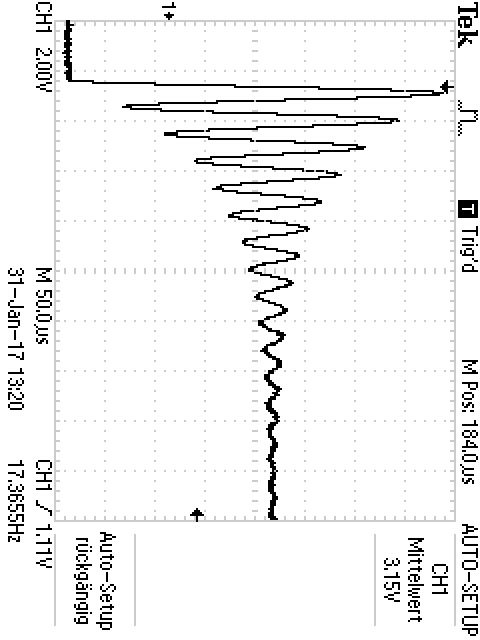
\includegraphics[width=\textwidth, angle=90, height=8cm]{F0001TEK.JPG}
  \caption{Gemessene Schwingungskurve.}
  \label{fig:Schwingungskurve}
\end{figure}

Die Schwingungskurve in Abb. \ref{fig:Schwingungskurve} wurde beim
Widerstand $R_1$ und einer Generatorfrequenz $\SI{5,82}{\hertz}$ erstellt.

Die diskreten Wertepaare ($U_C(t_i), t_i$) sind in der Tabelle \ref{tab:Messunga}
dargestellt. Dabei wurden für $U_C(t_i)$ jeweils die Maxima der Schwingungskurve
vermessen.

\floatplacement{table}{htbp}
\begin{table}
 \centering
 \sisetup{table-format=3.2}
 \begin{tabular}[width=\textwidth]{S S}
     \toprule
      {Zeit in $\si{\micro\second}$} & {Maxima in $\si{\volt}$} \\
     \midrule
      0 & 15,08 \\
      27,5 & 13,2 \\
      55 & 11,92 \\
      82,5 & 10,96 \\
      112,5 & 10,24 \\
      142,5 & 9,68 \\
      172,5 & 9,36 \\
      202,5 & 9,04 \\
      235 & 8,88 \\
      267,5 & 8,76 \\
      302,5 & 8,64 \\
      337,5 & 8,52 \\
      \bottomrule
  \end{tabular}
  \caption{Messdaten der Schwingungskurve.}
  \label{tab:Schwingungskurve}
\end{table}

Mit den Wertepaaren aus Tabelle \ref{tab:schwingungskurve} wurde mittels
des \emph{Python}-Paketes \emph{curve_fit} eine Ausgleichsrechnung an eine
exponential Funktion der Form

\begin{align}
  \label{eqn:exp}
  U_c(t) = a\cdot\exp^{-b\cdot t} + c
\end{align}

durchgeführt. Für die Parameter ergeben sich somit die Werte

\begin{align*}
  a & = \SI{6,62(3)}{\volt} \\
  b &= \num{1,17(1)e4}\frac{1}{\si{\per\second}} \\
  c &= \SI{8,44(2)}{\volt}
\end{align*}

Die Ausgleichfunktion ist mit den Daten aus Tabelle \ref{tab:Schwingungskurve} in Abb. \ref{fig:Ausgleichrechnung} dargestellt.

\begin{figure}
  \centering
  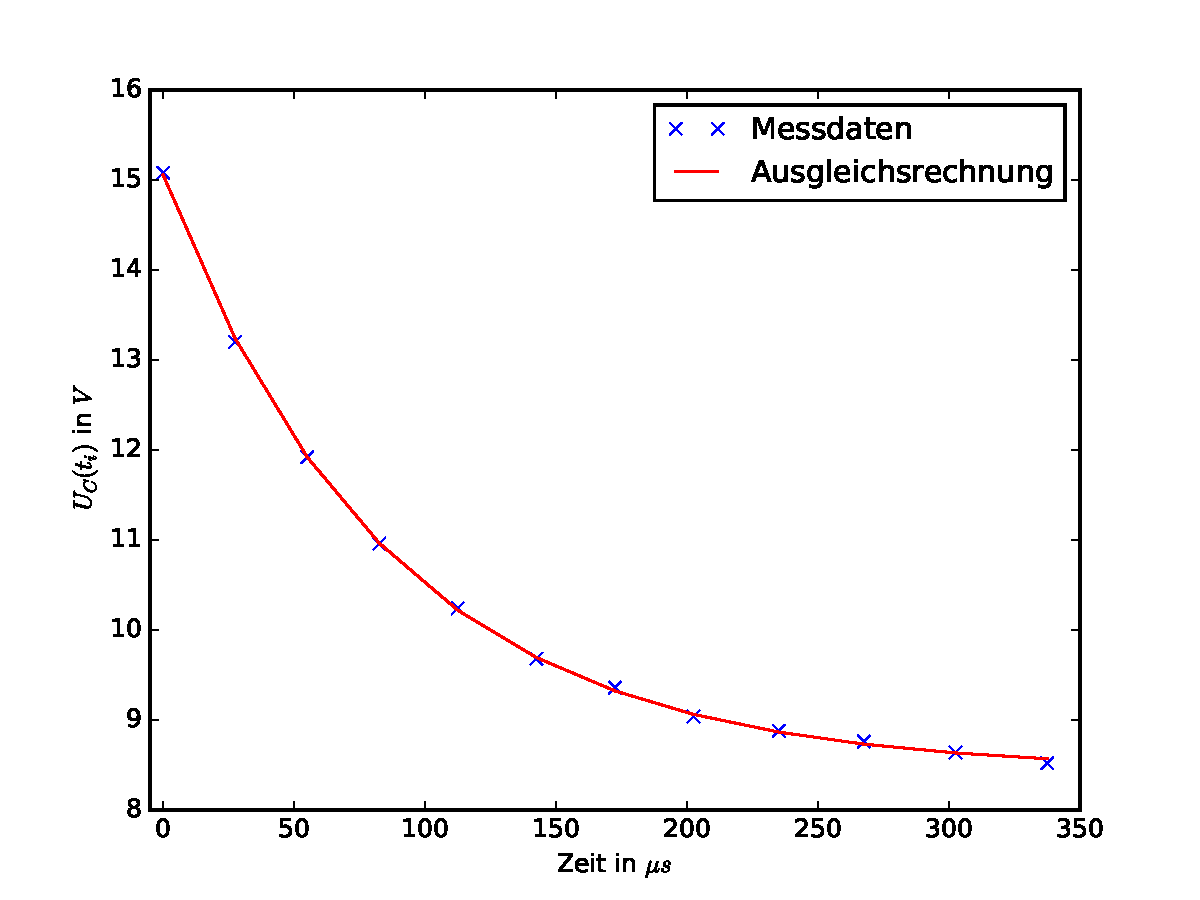
\includegraphics[width=\textwidth]{ausgleichsrechnung.pdf}
  \caption{Darstellung der Ausgleichsfunktion.}
  \label{fig:Ausgleichsrechnung}
\end{figure}

Der Exponent der Ausgleichsfunktion liefert über die Formeln (??) den
effektiv Widerstand $R_{eff}$ und die Abklingzeit $T_{ex}$.
Damit ergeben sich die folgenden Werte.

\begin{align*}
  R_{eff} &= \SI{82,4(12)}{\ohm}\\
  T_{ex} &= \SI{8,56(1)e-5}{\second}
\end{align*}

\end{document}
